\chapter{Estados}
\section{Introducción}
Los diagramas de estado son representaciones de los estados en los que puede estar un elemento. Estos son útiles para mostrar posibles situaciones en las que se puede encontrar un elemento,para mostrar las consecuencias y las condiciones para que haya cambios de estados y la direccionalidad (desde que estado se cambia a otro). Esta representación se utilizará en partes del programa donde haya un objeto que tenga diferentes estados, haya una transición entre ellos y sea importante tener conocimiento de ellos y sus consecuencias.

\section{Diagramas de estado}
Respecto al desarrollo que se lleva a cabo, se analizó y determinó que el objeto del que es necesario conocer sus estados , es el de tarea, pues hace parte fundamental en la solución del problema, así que el entendimiento de sus estados a lo largo de la ejecución del software que se pretende implementar será crucial.
\\
Los estados correspondientes para la tarea son:
\begin{itemize}
	\item Creada: Una tarea es  creada cuando el usuario la registra, pero aún no tiene un plazo definido para su realización.
	\item En proceso: La tarea se encuentra en proceso cuando ya se empezó a hacer y se está dentro del plazo de realización.
	\item Finalizada: La tarea está finalizada cuando ya se realizó la actividad.
\end{itemize}
El disparo para la acción es el proceso de la  tarea, que tiene en cuenta la fecha actual y la fecha de inicio y fin. Los efectos que suceden al cambiar de estado son:
\begin{itemize}
\item Iniciar tarea: La tarea pasa de estar creada estar en proceso, porque la fecha actual está en el rango de realizacion de la misma.
\item Terminar tarea: La tarea pasa al estado de finalizada porque la fecha actual es la fecha de terminación.
\item Cancelar tarea: La tarea también puede pasar a finalizada porque se canceló la tarea.
\item Aplazar tarea: Se puede pasar del estado finalizado al estado en proceso cuando se cambia el valor de la fecha de terminación a un posterior a la fecha actual.
\end{itemize}


\begin{figure}[H]
	\centering
	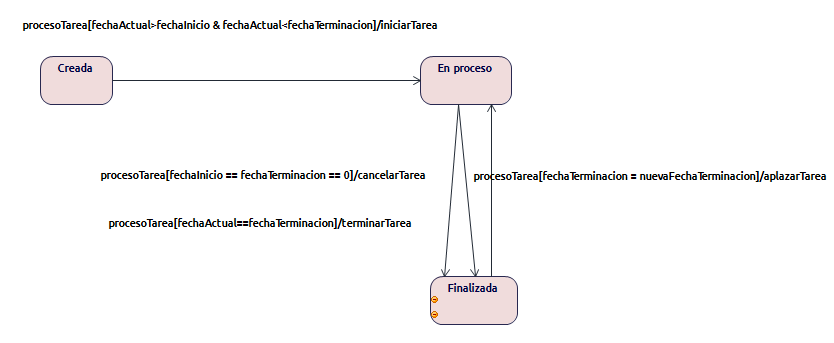
\includegraphics[width=1\linewidth]{diseno/estados/imgs/estadosTarea}
	\caption{Diagrama de estados para el objeto Tarea.}
	\label{fig:gantt}
\end{figure}

Cabe mencionar que este diagrama tendrá su representación en forma de diagrama de clase. Para esto, existe un patrón de comportamiento, que tiene como objetivo cumplir el principio de diseño abierto/cerrado en el contexto de estados de un objeto, ya que el diagrama de estados se representa en una sola clase,en cambio, el patrón estados, lo representa de tal forma que sea extensible y que no tenga que modificar la clase principal a la que afectan los estados. 

\begin{figure}[H]
	\centering
	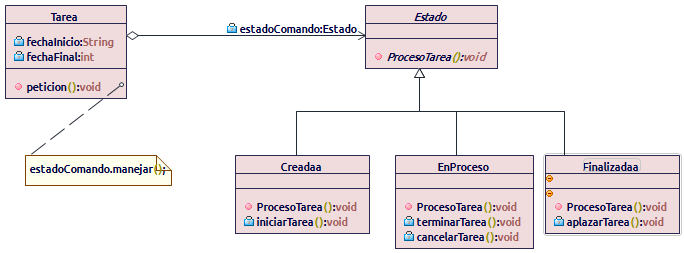
\includegraphics[width=1\linewidth]{diseno/estados/imgs/PatronState}
	\caption{Patrón state para solucionar los estados del objeto Tarea.}
	\label{fig:gantt}
\end{figure}

\begin{figure}[H]
	\centering
	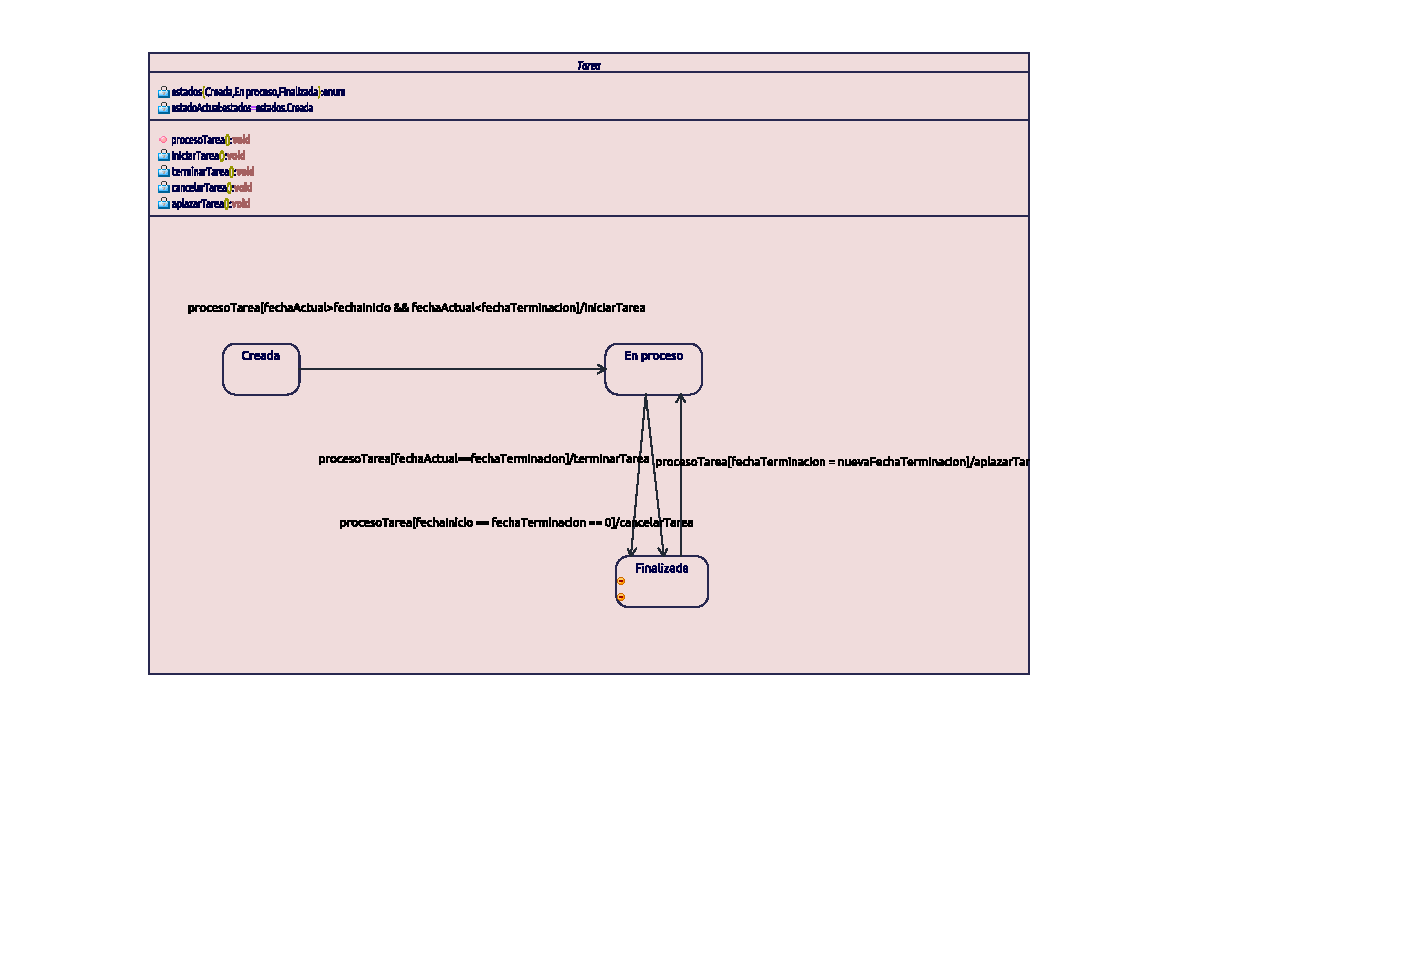
\includegraphics[width=1\linewidth]{diseno/estados/imgs/loquesea.pdf}
	\caption{Detalle de la clase Tarea bajo el contexto del patrón Estado.}
	\label{fig:gantt}
\end{figure}